\documentclass [12pt, executivepaper]{article}

\usepackage{mathtools}

\usepackage{outlines}

\usepackage{amsfonts}

\usepackage{booktabs}

\usepackage{graphicx}

\everymath{\displaystyle}

\usepackage{hyperref}

\usepackage{graphics}

\usepackage{commath}

\usepackage{adjustbox}

\begin{document}

\title {Technical Interview Prep Guide}
\author{Brendan Busey\\Wake Forest University\\ busebd12@wfu.edu}
\maketitle

\pagebreak

\vspace*{-40mm}

\section*{Complexity Analysis}

\begin{enumerate}

\item Big Oh Definitions:

\begin{enumerate}

\item $f(n)=\mathcal{O}(g(n))$ means $c \cdot g(n)$ is an upper bound on $f(n)$. Thus, there exists some constant $c$ such that $f(n)$ is always $\leq$ $c \cdot g(n)$, for large enough $n$

\item $f(n)=\Omega(g(n))$ means $c \cdot g(n)$ is a lower bound on $f(n)$. Thus, there exists some constant $c$ such that $f(n)$ is always $\geq$ $c \cdot g(n)$, for all $n$ $\geq$ $n_{0}$

\item $f(n)=\Theta(g(n))$ means $c_{1} \cdot g(n)$ is an upper bound on $f(n)$ and $c_{2} \cdot g(n)$ is a lower bound on $f(n)$, for all $n$ $\geq$ $n_{0}$. Thus, there exists constants $c_{1}$ and $c_{2}$ such that
$f(n) \leq c_{1} \cdot g(n)$ and $f(n) \geq c_{2} \cdot g(n)$. This means that $g(n)$ provides a nice, tight bound on $f(n)$.

\end{enumerate}

\item Tips on analysis:

\begin{enumerate}

\item If your algorithm is in the form "do this, then, when you're all done, do that," then you add the runtimes

\item If your algorithm is in the form "do this fo each time you do that," then you multiply the runtimes

\item Any algorithm that repeatedly doubles or halves, you should be thinking logarithmic complexity aka $\mathcal{O}(\log{} n)$
\item Amortized time allows us to describe that, yes, this worst case happens every once in a while. But, once this happens, it won't happen again for so long that the cost is "amortized"

\item When you have a recursive function that makes multiple calls, the runtime will often (but not always) look like $\mathcal{O}(branches^{depth})$, where branches is the number of times each recursive call branches aka 
how many times the recursive function is called

\item Memorization is a very common technique used to optimize exponential time recursive algorithms

\end{enumerate}

\end{enumerate}

\pagebreak

\vspace*{-40mm}

%%%%%%%%%%%%%%%%%%%%%%%%%%%%%%%%%%%%%%%%%%%%%%%%%START OF SORTING SECTION%%%%%%%%%%%%%%%%%%%%%%%%%%%%%%%%%%%%%%%%%%%%%%%%%%

\section*{Sorting}

%%%%%%%%%%START OF 	QUICKSORT%%%%%%%%
\begin{enumerate}

\item QuickSort

\begin{enumerate}

\item Complexity: $\mathcal{O}(n \log{} n)$

\item How it works:

\begin{enumerate}

\item Choose the pivot value: we take the value of the middle element as the pivot value, but it can be any value, which is in range of sorted values, even if it does appear in the array.

\item Partition: Rearrange elements in a such a way that all elements which are less than the pivot go the left part of the array and all elements greater than the pivot go to the right part of the array. Values equal to pivot can stay in any part of the array. Note, that the array may be divided into non-equal parts.

\item Sort both parts: apply Quicksort algorithm recursively to the left and right parts. 

\end{enumerate}

\item Advantage(s):

\begin{enumerate}

\item Fast and efficient for large data sets

\item Can carry out sequential traversal through array elements which results in good locality of reference and cache behaviour for arrays

\end{enumerate}

\item Disadvantage(s):

\begin{enumerate}

\item Not efficient if the elements are already sorted and if each element in the array are equal (gives worst case time complexity of $\mathcal{O}(n^2)$)

\item Might be space expensive for large data sets due to the fact that it uses $\mathcal{O}(\log{} n)$ auxiliary space for recursive function calls

\end{enumerate}

\pagebreak

\vspace*{-40mm}

\item Implementation

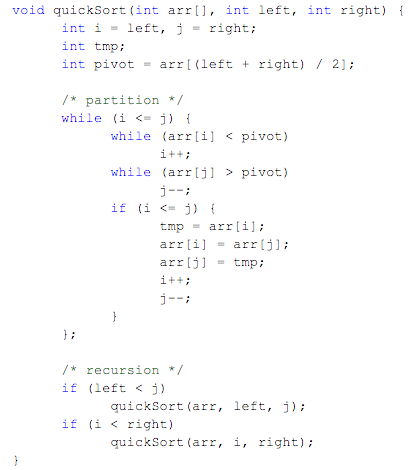
\includegraphics[scale=0.5]{QuickSort}

\end{enumerate}
%%%%%%%%%END OF QUICKSORT%%%%%%

%%%%%%%%%START OF MERGE SORT%%%%

\item Merge Sort

\begin{enumerate}

\item Complexity: $\mathcal{O}(n \log{} n)$

\item How it works:

\begin{enumerate}

\item We partition the elements into two groups, sorting each of the smaller problems recursively, and then interleaving the two sorted lists to totally order the elements

\end{enumerate}

\item Advantage(s):

\begin{enumerate}

\item Want to use it when the data is stored in a linked list, because merging does not require random access to the list elements

\end{enumerate}

\item Disadvantage(s):

\begin{enumerate}

\item Requires twice as much memory as than any other sophisticated sorting algorithm and likewise is not recommended for smaller arrays for the reason that it works recursively and it requires 
$\mathcal{O}(n)$ auxiliary space for sorting

\item It is difficult to implement the merge operation

\end{enumerate}

\pagebreak

\vspace*{-40mm}

\item Implementation

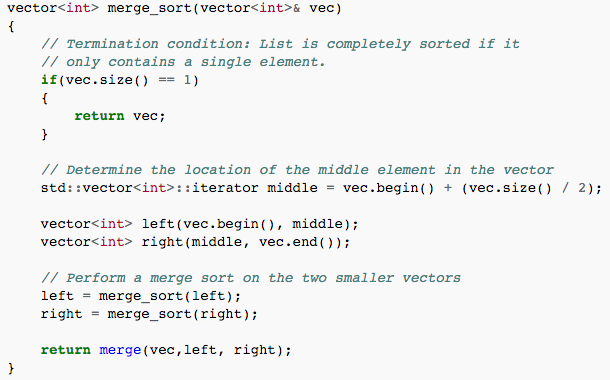
\includegraphics[scale=0.5]{MergeSortPart1}

\vspace{3mm}

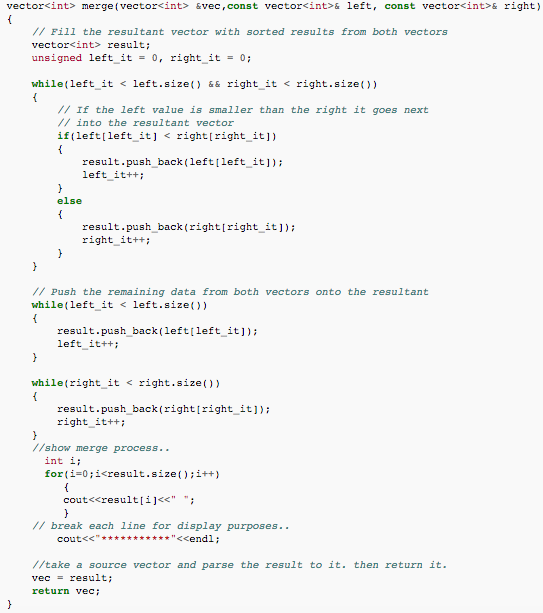
\includegraphics[scale=0.5]{MergeSortPart2}

\end{enumerate}
%%%%%%%%%END OF MERGE SORT%%%%%

\pagebreak

\vspace*{-40mm}

%%%%%%%%%START OF HEAP SORT%%%%%
\item Heap Sort

\begin{enumerate}

\item Complexity: $\mathcal{O}(n \log{} n)$

\item How it works:

\begin{enumerate}

\item It is similar to insertion sort where we first find the maximum element, exchange it with the last element, and then re-make the heap. We then repeat the process for the remaining elements.

\end{enumerate}

\item Advantage(s):

\begin{enumerate}

\item Used often for large data sets because it does not work recursively all the time

\end{enumerate}

\item Disadvantages(s):

\begin{enumerate}

\item Works slower than other sorting methods with the same computational complexity

\item Not efficient for parallelization

\item Not recommended for sorting data that is stored in a linked list because it is difficult to convert a linked list into a heap like structure

\end{enumerate}

\end{enumerate}
%%%%%%%%%END OF HEAP SORT%%%%%%
\end{enumerate}
%%%%%%%%%%%%%%%%%%%%%%%%%%%%%%%%%%%%%%%%%%%%%%%%%END OF SORTING SECTION%%%%%%%%%%%%%%%%%%%%%%%%%%%%%%%%%%%%%%%%%%%%%%%%%%%

\pagebreak

\vspace*{-40mm}

%%%%%%%%%%%%%%%%%%%%%%%%%%%%%%%%%%%%%%%%%%%%%%%%%START OF HASH TABLE SECTION%%%%%%%%%%%%%%%%%%%%%%%%%%%%%%%%%%%%%%%%%%%%%%%%

\section*{Hash Table(s)}

\begin{enumerate}

\item How do they work?

\begin{enumerate}

\item Let's assume you want to fill up a library of books and not just stuff them in there, but you want to be able to easily find them again when you need them.\\

So, you decide that if the person that wants to read a book knows the title of the book and the exact title to boot, then that's all it should take. With the title, the person, with the aid of the librarian, should be able to find the book easily and quickly. \\

So, how can you do that? Well, obviously you can keep some kind of list of where you put each book, but then you have the same problem as searching the library, you need to search the list. Granted, the list would be smaller and easier to search, but still you don't want to search sequentially from one end of the library (or list) to the other.\\

You want something that, with the title of the book, can give you the right spot at once, so all you have to do is just stroll over to the right shelf, and pick up the book.\\

But how can that be done? Well, with a bit of forethought when you fill up the library and a lot of work when you fill up the library.\\

Instead of just starting to fill up the library from one end to the other, you devise a clever little method. You take the title of the book, run it through a small computer program, which spits out a shelf number and a slot number on that shelf. This is where you place the book.\\

\pagebreak 

\vspace*{-40mm}

The beauty of this program is that later on, when a person comes back in to read the book, you feed the title through the program once more, and get back the same shelf number and slot number that you were originally given, and this is where the book is located.\\

The program is called a hash algorithm or hash computation and usually works by taking the data fed into it (the title of the book in this case) and calculates a number from it.\\

For simplicity, let's say that it just converts each letter and symbol into a number and sums them all up. In reality, it's a lot more complicated than that, but let's leave it at that for now.\\

The beauty of such an algorithm is that if you feed the same input into it again and again, it will keep spitting out the same number each time.\\

Ok, so that's basically how a hash table works.

\end{enumerate}

\item Implementation: Know your implementation like the back of your hand and study up on the ones provided by the C++ STL

\item Complexities

\begin{enumerate}

\item Insertion: $\mathcal{O}(1)$

\item Deletion: $\mathcal{O}(1)$

\item Search: $\mathcal{O}(1)$

\end{enumerate}

\end{enumerate}
%%%%%%%%%%%%%%%%%%%%%%%%%%%%%%%%%%%%%%%%%%%%%%%%%END OF HASH TABLE SECTION%%%%%%%%%%%%%%%%%%%%%%%%%%%%%%%%%%%%%%%%%%%%%%%%%

\pagebreak

\vspace*{-40mm}

%%%%%%%%%%%%%%%%%%%%%%%%%%%%%%%%%%%%%%%%%%%%%%%%%START OF TREE SECTION%%%%%%%%%%%%%%%%%%%%%%%%%%%%%%%%%%%%%%%%%%%%%%%%%%%%
\section*{Tree(s)}

\begin{enumerate}

%%%%%%%%%START OF BINARY TREE SECTION%%%%%%%%%%
\item Binary Trees

\begin{enumerate}

\item A data structure in which each node has two children, a left and right child

\item Major Algorithms

\begin{enumerate}

\item Pre-order traversal (Type of depth first traversal/search)

\begin{enumerate}

\item Visit order: root, left child, right child

\item Complexity: $\mathcal{O}(n)$, where $n$ is the number of nodes in your tree

\end{enumerate}

\item In-order traversal (type of depth first search/traversal)

\begin{enumerate}

\item Visit order: left child, root, right child

\item Complexity: $\mathcal{O}(n)$, where $n$ is the number of nodes in your tree

\end{enumerate}

\item Post-order traversal (type of depth first search/traversal)

\begin{enumerate}

\item Visit order: left child, right child, root

\item Complexity: $\mathcal{O}(n)$, where $n$ is the number of nodes in your tree

\end{enumerate}

\item Breadth First Traversal/Search

\begin{enumerate}

\item How it works: traverses the tree one level at a time, left to right within a level 

\item Time complexity: $\mathcal{O}(n)$, where $n$ is the number of nodes since you have to visit all the nodes in the tree

\item Space complexity: $\mathcal{O}(n)$, where $n$ is the number of nodes since you have to hold all of the nodes in a queue

\item Implementation:

\vspace{1mm}

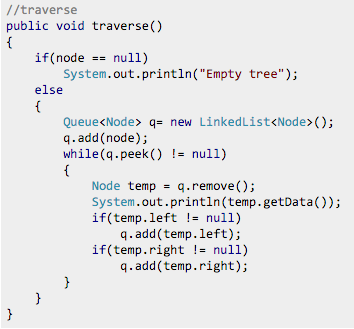
\includegraphics[scale=0.5]{BreadthFirstTraversalForTree}

\end{enumerate}

\end{enumerate}

\end{enumerate}
%%%%%%%END OF BINARY TREE SECTION%%%%%%%%

\pagebreak

\vspace*{-40mm}

%%%%%%%START OF N-ARY TREE SECTION%%%%%%%
\item $N$-ary Trees

\begin{enumerate}

\item Is a data structure that consists of a root node and then $N$ subtrees

\item Major Algorithms

\begin{enumerate}

\item Pre-order traversal

\begin{enumerate}

\item Print out the current node, then loop through the children of the current node and recursively call the pre-order traversal function on each of them

\item Complexity: $\mathcal{O}(n)$, where $n$ is the number of nodes since you have to visit all the nodes in the tree

\end{enumerate}

\item Post-order traversal

\begin{enumerate}

\item Loop through the children of the current node and recursively call the post-order traversal function on each of them, then print out the current node

\item Complexity: $\mathcal{O}(n)$, where $n$ is the number of nodes since you have to visit all the nodes in the tree

\end{enumerate}

\item Breadth First Search

\vspace{1mm} 

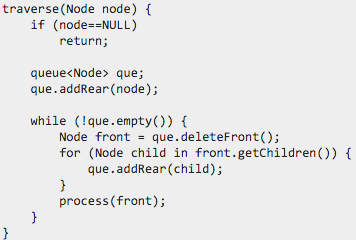
\includegraphics[scale=0.5]{BreadthFirstSearchN-aryTree}

\begin{enumerate}

\item Complexity: $\mathcal{O}(n)$, where $n$ is the number of nodes since you have to visit all the nodes in the tree

\end{enumerate}

\item Depth First Search

\vspace{1mm}

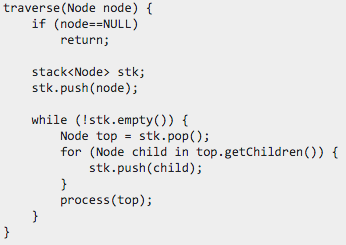
\includegraphics[scale=0.5]{DepthFirstSearchN-aryTree}

\pagebreak

\vspace*{-40mm}

\begin{enumerate}

\item Complexity: $\mathcal{O}(n)$, where $n$ is the number of nodes since you have to visit all the nodes in the tree

\end{enumerate}

\item Implementation: each node will have data associated with it as well as a vector to store it's $n$ other childen

\end{enumerate}

\end{enumerate}
%%%%%%%END OF N-ARY TREE SECTION%%%%%%%%

%%%%%%%START OF TRIE SECTION%%%%%%%%%%%

\item Trie(s)

\begin{enumerate}

\item A tree where every vertex represents either a word or prefix

\item Major Algorithms:

\begin{enumerate}

\item Similar to those for $N$-ary trees

\end{enumerate}

\item Implementation: identical to that of a $N$-ary tree except that you will be storing characters in the vector

\end{enumerate}
%%%%%%%END OF TRIE SECTION%%%%%%%%%%%%

%%%%%%%START OF AVL TREE SECTION%%%%

\item AVL Tree(s)

\begin{enumerate}

\item Is a binary search tree with the following properties:

\begin{enumerate}

\item The sub-tree(s) of every node differ in height by exactly one

\item Every sub-tree is also an AVL tree

\end{enumerate}

\item Why do we care about AVL tree(s)?

\begin{enumerate}

\item Most of the BST operations (e.g., search, max, min, insert, delete.. etc) take $\mathcal{O}(h)$ time where $h$ is the height of the BST. The cost of these operations may become $\mathcal{O}(n)$ for a skewed Binary tree. 
If we make sure that height of the tree remains $\mathcal{O}(\log{} n)$ after every insertion and deletion, then we can guarantee an upper bound of $\mathcal{O}(\log{} n)$ for all these operations. 

\end{enumerate}

\item Insertion process for a node $n$

\begin{enumerate}

\item Perform the standard Binary Search Tree insertion for $n$

\item Starting from $n$, travel up in the tree until we find the first unbalanced node, call it $z$

\item Re-balance the tree by performing the appropriate rotations for the sub-tree with root $z$

\pagebreak

\vspace*{-40mm}

\item There are four possible cases to consider for re-balancing:

\begin{enumerate}

\item Case $1$: Left Left

\vspace{2mm}

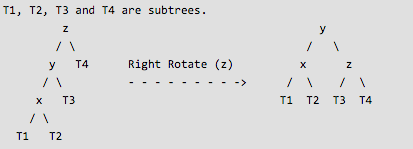
\includegraphics[scale=0.5]{RotationCase1AVLTree}

\item Case $2$: Left Right

\vspace{2mm}

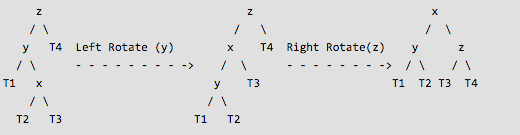
\includegraphics[scale=0.5]{RotationCase2AVLTree}

\item Case $3$: Right Right

\vspace{2mm}

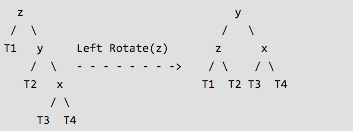
\includegraphics[scale=0.5]{RotationCase3AVLTree}

\item Case $4$: Right Left

\vspace{2mm}

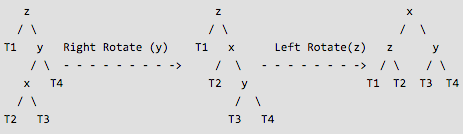
\includegraphics[scale=0.5]{RotationCase4AVLTree}

\end{enumerate}

\item Implementation for insertion:

\begin{enumerate}

\item Perform the normal Binary Search Tree insertion

\item The current node must be one of the ancestors of the newly inserted node. Update the height of the current node.

\item Get the balance factor (left subtree height - right subtree height)

\item If balance factor is greater than $1$, then the current node is unbalanced and we are either in Left Left case or left Right case. We are in the Left Left case if the newly inserted key is less than the key of its left sub-tree. We are in the Left Right case if the newly inserted key is greater than the key of its left sub-tree.

\pagebreak

\vspace*{-40mm}

\item If balance factor is less than $-1$, then the current node is unbalanced and we are either in Right Right case or Right Left case. We are in the Right Right case if the newly inserted key is greater than the key of its right sub-tree. We are in the Right Left case if the newly inserted key is less than the key of its right sub-tree.

\end{enumerate}

\end{enumerate}

\item Deletion process for a node $n$

\begin{enumerate}

\item Perform the normal deletion for Binary Search Tree

\item Starting from $n$, travel up in the tree until we find the first unbalanced node, call it $z$

\item Re-balance the tree by performing the appropriate rotations for the sub-tree with root $z$

\item There are four cases to consider for re-balancing:

\begin{enumerate}

\item Case $1$: Left Left

\vspace{2mm}

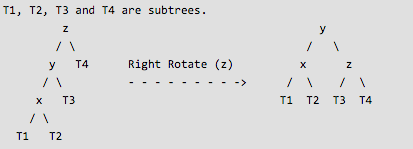
\includegraphics[scale=0.5]{RotationCase1AVLTree}

\item Case $2$: Left Right

\vspace{2mm}

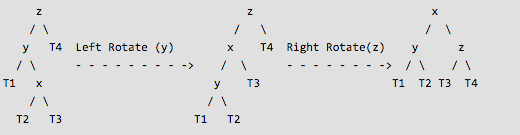
\includegraphics[scale=0.5]{RotationCase2AVLTree}

\item Case $3$: Right Right

\vspace{2mm}

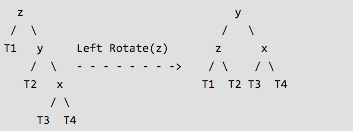
\includegraphics[scale=0.5]{RotationCase3AVLTree}

\item Case $4$: Right Left

\vspace{2mm}

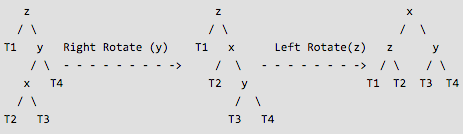
\includegraphics[scale=0.5]{RotationCase4AVLTree}

\end{enumerate}

\pagebreak

\vspace*{-40mm}

\item Implementation for deletion:

\begin{enumerate}

\item Perform the normal Binary Search Tree deletion

\item The current node must be one of the ancestors of the deleted node; update the height of the current node

\item Get the balance factor (left subtree height - right subtree height) of the current node

\item If balance factor is greater than $1$, then the current node is unbalanced and we are either in Left Left case or Left Right case. To check whether it is Left Left case or Left Right case, get the balance factor of left subtree. If balance factor of the left subtree is greater than or equal to $0$, then it is Left Left case, else Left Right case.

\item If balance factor is less than $-1$, then the current node is unbalanced and we are either in Right Right case or Right Left case. To check whether it is Right Right case or Right Left case, get the balance factor of right subtree. If the balance factor of the right subtree is smaller than or equal to $0$, then it is Right Right case, else Right Left case.

\end{enumerate}

\end{enumerate}

\end{enumerate}
%%%%%%%END OF AVL TREE SECTION%%%%%

%%%%%%%START OF BREADTH FIRST AND DEPTH FIRST COMPARISON SECTION%%%%%
\item Breadth First and Depth First Comparison

\begin{enumerate}

\item When to use Breadth First

\begin{enumerate}

\item If you know what you want to search for is not far from the root

\item If the tree is very deep and solutions are not very common 

\end{enumerate}

\item When to use Depth First

\begin{enumerate}

\item If the tree is wide, since breadth first might take up too much memory

\item If solutions are frequent and located deep in the tree, breadth first might take too long

\end{enumerate}

\item Complexities

\begin{enumerate}

\item Breadth First: $\mathcal{O}(n)$

\item Depth First: $\mathcal{O}(n)$

\end{enumerate}

\end{enumerate}
%%%%%%%END OF BREADTH FIRST AND DEPTH FIRST COMPARISON SECTION%%%%%%

\end{enumerate}
%%%%%%%%%%%%%%%%%%%%%%%%%%%%%%%%%%%%%%%%%%%%%%%%%END OF TREE SECTION%%%%%%%%%%%%%%%%%%%%%%%%%%%%%%%%%%%%%%%%%%%%%%%%%%%%%

\pagebreak

\vspace*{-40mm}

%%%%%%%%%%%%%%%%%%%%%%%%%%%%%%%%%%%%%%%%%%%%%%%%%START OF GRAPH SECTION%%%%%%%%%%%%%%%%%%%%%%%%%%%%%%%%%%%%%%%%%%%%%%%%%%%
\section*{Graphs}

\begin{enumerate}

\item Adjacency Matrix Representation

\begin{enumerate}

\item is a 2D array of size $V$ x $V$ where $V$ is the number of vertices in a graph

\item Complexity:

\begin{enumerate}

\item Adding an edge $\rightarrow \mathcal{O}(1)$

\item Deleting an edge $\rightarrow \mathcal{O}(1)$

\item Answering the question "is there an edge between two vertices" $\rightarrow \mathcal{O}(1)$

\item Finding the successors of a given vertex $\rightarrow \mathcal{O}(n)$

\item Determining if a path exists between two vertices $\rightarrow \mathcal{O}(n^2)$

\end{enumerate}

\item Advantage(s):

\begin{enumerate}

\item Representation is easier to implement and follow

\item Removing and edge takes constant time

\item Answering the question "is there an edge between two vertices" can be answered in constant time

\end{enumerate}

\item Disadvantage(s):

\begin{enumerate}

\item Space complexity is $\mathcal{O}(V^2)$, where $V$ is the number of vertices

\item Even if the graph is sparse, still takes up $\mathcal{O}(V^2)$ space

\item Adding a vertex is $\mathcal{O}(V^2)$ time

\end{enumerate}

\end{enumerate}

\item Adjacency List Representation

\begin{enumerate}

\item We keep a list of all vertices and each vertex within that list has its own list that contains their adjacent vertices

\item Complexity:

\begin{enumerate}

\item Adding an edge $\rightarrow \mathcal{O}(\log{} V)$

\item Deleting an edge $\rightarrow \mathcal{O}(\log{} V)$

\item Answer the questions "is there an edge between two vertices"  $\rightarrow \mathcal{O}(\log{} V)$

\item Finding the successor of a given vertex $\rightarrow \mathcal{O}(\log{} n)$, where $n$ is the length of the lists containing the successors of a given vertex

\pagebreak

\vspace*{-40mm}

\item Determining if a path exists between two vertices $\rightarrow \mathcal{O}(V+E)$, where $V$ is number of vertices and $E$ is the number of edges

\end{enumerate}

\item Advantage(s):

\begin{enumerate}

\item Saves space; average space complexity is $\mathcal{O}(V+E)$; worst case is $\mathcal{O}(V^2)$

\item Adding a vertex is easier

\end{enumerate}

\item Disadvantage(s):

\begin{enumerate}

\item Queries like whether there is an edge from vertex $u$ to vertex $v$ are not efficient and can be done $\mathcal{O}(V)$, where $V$ is the number of vertices

\end{enumerate}

\end{enumerate}

\item Major Algorithms

\begin{enumerate}

\item Breadth First Traversal

\begin{enumerate}

\item Complexity: $\mathcal{O}(V+E)$, where $V$ is the number of vertices and $E$ is the number of edges

\item Implementation:

\vspace{1mm}

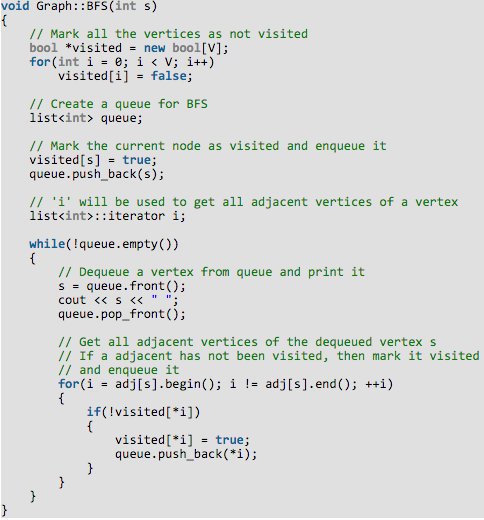
\includegraphics[scale=0.5]{BreadthFirstSearchForGraph}

\end{enumerate}

\pagebreak

\vspace*{-40mm}

\item Depth First Search

\begin{enumerate}

\item Complexity: $\mathcal{O}(V+E)$, where $V$ is the number of vertices and $E$ is the number of edges

\item Implementation:

\vspace{1mm}

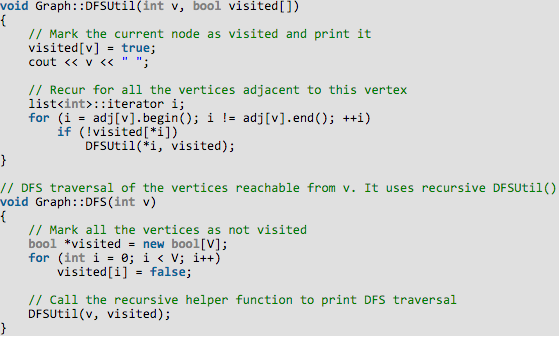
\includegraphics[scale=0.5]{DepthFirstSearchGraph}

\vspace{3mm}

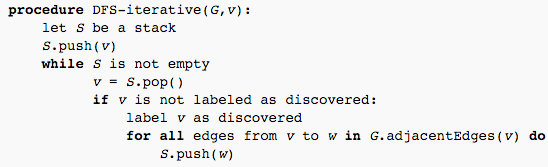
\includegraphics[scale=0.5]{DepthFirstSearchGraphIterative}

\end{enumerate}

\item Dijkstra's Algorithm

\begin{enumerate}

\item Description:

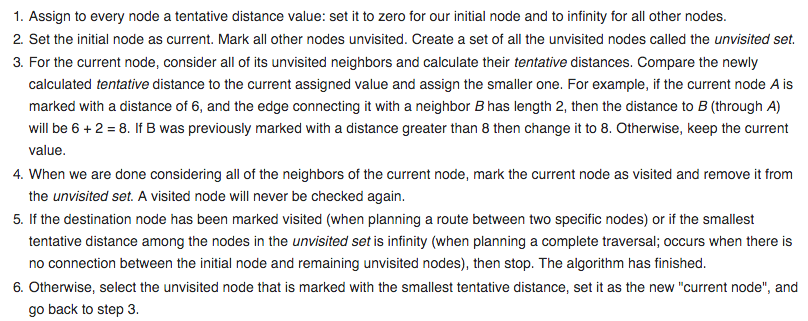
\includegraphics[scale=0.4]{DijkstraAlgorithmDescription}

\pagebreak

\vspace*{-40mm}

\item Implementation:

\vspace{1mm}

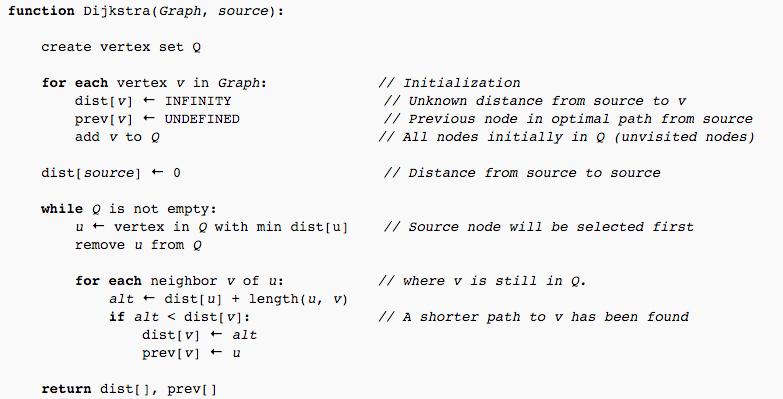
\includegraphics[scale=0.4]{DijkstraPseudoCode}

\end{enumerate}

\item A* Algorithm

\begin{enumerate}

\item A* is like Dijkstra's algorithm in that it can be used to find a shortest path

\item A* is like Greedy Best-First-Search in that it can use a heuristic to guide itself

\item The secret to its success is that it combines the pieces of information that Dijkstra?s algorithm uses (favoring vertices that are close to the starting point) and information that Greedy Best-First-Search uses (favoring vertices that are close to the goal)

\item When talking about the algorithm, $g(n)$ represents the exact cost of the path from the starting point to any vertex $n$

\item When talking about the algorithm, $h(n)$ represents the heuristic estimated cost from vertex n to the goal

\end{enumerate}

\end{enumerate}

\end{enumerate}
%%%%%%%%%%%%%%%%%%%%%%%%%%%%%%%%%%%%%%%%%%%%%%%%%END OF GRAPH SECTION%%%%%%%%%%%%%%%%%%%%%%%%%%%%%%%%%%%%%%%%%%%%%%%%%%%%%

%%%%%%%%%%%%%%%%%%%%%%%%%%%%%%%%%%%%%%%%%%%%%%START OF NP-COMPLETE PROBLEM(S) SECTION%%%%%%%%%%%%%%%%%%%%%%%%%%%%%%%%%%%%%%%%%%%
\section*{NP-Complete Problem(s)}

\begin{enumerate}

\item NP stands for Non-deterministic Polynominal time

\item A yes-or-no problems is said to be NP if a yes can be verified in polynominal time

\item NP-complete is a family of NP problems for which you know that if one had a polynominal time solution, then everyone of them has a polynominal time solution

\item Some famous examples of NP problems:

\pagebreak

\vspace*{-40mm}

\begin{enumerate}

\item Traveling Salesman problem: finding the shortest path (on a graph) that allows you to visit each city exactly once

\item Bin packing problem: there are a number of fixed (integer) size bins and objects of varying sizes. Minimize the number of bins required to hold all of the object

\item Knapsack problem: given objects of various sizes and values and a knapsack with a fixed integer size, choose the objects that can fit inside with the most value

\item Minimal Vertex Cover: finding the smallest set of vertices such that every edge contains at least one chosen vertex

\item Clique: finding that largest group of people who all know each other

\item Subgraph Isomorphism: does one graph contain a subgraph isomorphic to another?

\item Set packing: given a number of sets, what is the maximum number of disjoint sets that can be selected? This is related to set cover, where we are trying to choose sets so that every element is within at least one set

\item Subset sum: Given a set of integers, does some subset sum to 0?

\end{enumerate}

\end{enumerate}
%%%%%%%%%%%%%%%%%%%%%%%%%%%%%%%%%%%%%%%%%%%%%%END OF NP-COMPLETE PROBLEM(S) SECTION%%%%%%%%%%%%%%%%%%%%%%%%%%%%%%%%%%%%%%%%%%%%

\pagebreak

\vspace*{-40mm}

%%%%%%%%%%%%%%%%%%%%%%%%%%%%%%%%%%%%%%%%%%%%%%START OF OPERATING SYSTEM SECTION%%%%%%%%%%%%%%%%%%%%%%%%%%%%%%%%%%%%%%%%%%%%%%%
\section*{Operating Systems}

\begin{enumerate}

\item Process: an instance of computer program in execution

\item Thread: a basic unit of CPU utilization, often called a "lightweight" process

\item Concurrency issues

\begin{enumerate}

\item Race condition(s): behaviour of software or system where the output is dependent on the sequence or timing of other uncontrollable events  

\item Deadlock: a specific condition when two or more processes are each waiting for another to release a resource, or more than two processes are waiting for resources in a circular chain

\item Livelock: similar to a deadlock, except that the states of the processes involved in the livelock constantly change with regard to one another, none progressing

\end{enumerate}

\item Lock(s): something that programmers annotate source code with, especially critical sections, to ensure that any such critical section executes as if it was a single atomic instruction

\item Mutex(es): used to serialise access to a section of  re-entrant code that cannot be executed concurrently by more than one thread

\begin{enumerate}

\item Real world example: Imagine a mutex as a key to a toilet. One person can have the key - occupy the toilet - at the time. When they are finished, the person gives (frees) the key to the next person in the queue

\end{enumerate} 

\item Semaphore(s): something that restricts the number of simultaneous users (threads) of a shared resource up to a maximum number

\begin{enumerate}

\item Real world example: Going back to our earlier toilet example, a semaphore is the number of free identical toilet keys. Say we have four toilets with identical locks and keys. The semaphore count - the count of keys - is set to 4 at beginning (all four toilets are free), then the count value is decremented as people are coming in. If all toilets are full, ie. there are no free keys left, the semaphore count is 0. 

\pagebreak

\vspace*{-40mm}

Now, when one person leaves the toilet, semaphore is increased to 1 (one free key), and given to the next person in the queue

\end{enumerate}

\item Monitor(s): A monitor is a set of multiple routines which are protected by a mutual exclusion lock

\begin{enumerate}

\item Four main components:

\begin{enumerate}

\item Initialization: contains the code that is used exactly once when the monitor is created

\item Private data: private data, including private procedures, that can only be used within the monitor

\item Monitor procedure(s): procedures that can be called from outside of the monitor

\item Entry queue: contains all threads that called monitor procedures but have not been granted permissions 

\end{enumerate}

\end{enumerate}

\item Deadlock

\begin{enumerate}

\item Technical definition: a specific condition when two or more processes are each waiting for another to release a resource, or more than two processes are waiting for resources in a circular chain

\item Real world example: imagine two children are rummaging through a toy box because they want to play with a drum. However, one child finds the drumstick while the other finds the actual drum. Now, both children want to play with the drum but in order for this to happen, either the child with the drumstick has to give up the drumstick or the child with the drum has to give up the drum. Of course, since both children want to play with the drum, neither is going to do this, so both will be waiting forever for the other to give up what they have.

\end{enumerate}

\item Livelock

\begin{enumerate}

\item Technical definition: similar to a deadlock, except that the states of the processes involved in the livelock constantly change with regard to one another, none progressing

\item Real world example: two people meet in a narrow corridor, and each tries to be polite by moving aside to let the other pass, but they end up swaying from side to side without making any progress because they both repeatedly move the same way at the same time

\end{enumerate}

\pagebreak

\vspace*{-40mm}

\item What resources does a thread need?

\begin{enumerate}

\item Process ID

\item Program counter

\item Function stack

\item Set of registers

\end{enumerate}

\item What resources does a process need?

\begin{enumerate}

\item Process Control Block

\begin{enumerate}

\item Process state: new, ready, running, waiting, terminating

\item Process ID and parent process ID

\item CPU registers and program counter

\item CPU scheduling information such as priority information and pointers to scheduling queues

\item Memory management information such as page tables or segment tables 

\item Accounting information such as user and kernel CPU time consumed, account numbers, limits, etc

\item I/O status information such as Devices allocated, open file tables, etc

\end{enumerate}

\end{enumerate}

\item Context Switching

\begin{enumerate}

\item What is it?

\begin{enumerate}

\item Context switching is the process of switching a process from working on one task to working on another even before the former task is completed

\end{enumerate}

\item What does it involve?

\begin{enumerate}

\item This involves saving the state of all volatile data like registers, program counter, memory, etc. (in other words the "context" of the process)  to persistent storage and then loading up the context of a new process

\end{enumerate}

\item Before we get to process switching, we have to talk about the steps in thread context switching:

\pagebreak

\vspace*{-40mm}

\begin{enumerate}

\item All context switches are initiated by an 'interrupt'. This could be an actual hardware interrupt that runs a driver, (eg. from a network card, keyboard, memory-management or timer hardware), or a software call, (system call), that performs a hardware-interrupt-like call sequence to enter the OS

\item Non-trivial systems will have to initiate a hardware-protection-level change to enter a kernel-state so that the kernel code/data etc. can be accessed

\item Core state for the interrupted thread has to be saved. On a simple embedded system, this might just be pushing all registers onto the thread stack and saving the stack pointer in its Thread Control Block

\item Many systems switch to an OS-dedicated stack at this stage so that the bulk of OS-internal stack requirements are not inflicted on the stack of every thread

\item It may be necessary to mark the thread stack position where the change to interrupt-state occurred to allow for nested interrupts

\item The driver/system call runs and may change the set of ready threads by adding/removing TCB's from internal queues for the different thread priorities, eg. network card driver may have set an event or signaled a semaphore that another thread was waiting on, so that thread will be added to the ready set, or a running thread may have called sleep() and so elected to remove itself from the ready set

\item The OS scheduler algorithm is run to decide which thread to run next, typically the highest-priority ready thread that is at the front of the queue for that priority

\item The saved stack pointer from the TCB for that thread is retrieved and loaded into the hardware stack pointer

\item The core state for the selected thread is restored. On my simple system, the registers would be popped from the stack of the selected thread. More complex systems will have to handle a return to user-level protection

\item An interrupt-return is performed, so transferring execution to the selected thread

\end{enumerate}

\item Okay, now that we have talked about thread context switching, we can now talk about the steps in process context switching:

\pagebreak

\vspace*{-40mm}

\begin{enumerate}

\item Process context switches are initiated by a thread-context switch, so all of the above, 1-9, is going to need to happen

\item At step 5 in the thread context switching process, the scheduler decides to run a thread belonging to a different process from the one that owned the previously-running thread

\item The memory-management hardware has to be loaded with the address-space for the new process, ie whatever selectors/segments/flags/whatever that allow the thread/s of the new process to access its memory

\item The context of any Floating Point Unit  hardware needs to be saved/restored from the Process Control Block

\item There may be other process-dedicated hardware that needs to be saved/restored

\end{enumerate}

\end{enumerate}

\end{enumerate}
%%%%%%%%%%%%%%%%%%%%%%%%%%%%%%%%%%%%%%%%%%%%%%END OF OPERATING SYSTEM SECTION%%%%%%%%%%%%%%%%%%%%%%%%%%%%%%%%%%%%%%%%%%%%%%%%

%%%%%%%%%%%%%%%%%%%%%%%%%%%%%%%%%%%%%%%%%%%%%%START OF COMPLEXITIES SECTION%%%%%%%%%%%%%%%%%%%%%%%%%%%%%%%%%%%%%%%%%%%%%%%%%%
\section*{Complexities}

Data structures

\vspace{3mm}

\begin{adjustbox}{max height=6in, max width=6in}

    \begin{tabular}{l*{6}{c}r}
    
    Data Structure & Access (average) & Search (average) & Insertion (average) & Deletion (average) & Space \\
    
    \hline
    
    Singly-Linked List & $\mathcal{O}(n)$ & $\mathcal{O}(n)$ & $\mathcal{O}(1)$ & $\mathcal{O}(1)$ & $\mathcal{O}(n)$  \\
    
    Doubly-Linked List & $\mathcal{O}(n)$ & $\mathcal{O}(n)$ & $\mathcal{O}(1)$ & $\mathcal{O}(1)$ & $\mathcal{O}(n)$  \\
    
    Array & $\mathcal{O}(1)$ & $\mathcal{O}(n)$ & $\mathcal{O}(n)$ & $\mathcal{O}(n)$ & $\mathcal{O}(n)$  \\
    
    Stack & $\mathcal{O}(n)$ & $\mathcal{O}(n)$ & $\mathcal{O}(1)$ & $\mathcal{O}(1)$ & $\mathcal{O}(n)$  \\
    
    Queue & $\mathcal{O}(1)$ & $\mathcal{O}(n)$ & $\mathcal{O}(1)$ & $\mathcal{O}(1)$ & $\mathcal{O}(n)$  \\
    
    Binary Tree & $\mathcal{O}(\log{} n)$ & $\mathcal{O}(\log{} n)$ & $\mathcal{O}(\log{} n)$ & $\mathcal{O}(\log{} n)$ & $\mathcal{O}(n)$  \\
    
    AVL Tree & $\mathcal{O}(\log{} n)$ & $\mathcal{O}(\log{} n)$ & $\mathcal{O}(\log{} n)$ & $\mathcal{O}(\log{} n)$ & $\mathcal{O}(n)$
    
    \end{tabular}
    
\end{adjustbox}

\vspace{3mm}

\hspace{-8mm} Algorithms

\vspace{3mm}

\begin{adjustbox}{max height=4in, max width=4in}

    \begin{tabular}{l*{6}{c}r}
    
    Algorithm & Time & Space \\
    
    \hline
    
   Quicksort & $\mathcal{O}(n \log{} n)$ & $\mathcal{O}(\log{} n)$  \\
    
   Mergesort & $\mathcal{O}(n \log{} n)$ & $\mathcal{O}(n)$  \\
    
   Heapsort & $\mathcal{O}(\log{} n)$ & $\mathcal{O}(1)$ \\
    
   Depth First Search (Trees) & $\mathcal{O}(n)$ & $\mathcal{O}(n)$  \\
    
   Breadth First Search (Trees) & $\mathcal{O}(n)$ & $\mathcal{O}(n)$  \\
    
   Depth First Search (Graph(s)) & $\mathcal{O}(\abs{V} + \abs{E})$ & $\mathcal{O}(\abs{V})$  \\
    
   Breadth First Search (Graph(s)) & $\mathcal{O}(\abs{V} + \abs{E})$ & $\mathcal{O}(\abs{V})$
    
    \end{tabular}
    
\end{adjustbox}
%%%%%%%%%%%%%%%%%%%%%%%%%%%%%%%%%%%%%%%%%%%%%%END OF COMPLEXITIES SECTION%%%%%%%%%%%%%%%%%%%%%%%%%%%%%%%%%%%%%%%%%%%%%%%%%%%

\pagebreak

\vspace*{-40mm}

%%%%%%%%%%%%%%%%%%%%%%%%%%%%%%%%%%%%%%%%%%%%%%START OF REFERENCE SECTION%%%%%%%%%%%%%%%%%%%%%%%%%%%%%%%%%%%%%%%%%%%%%%%%%%%
\begin{center}

\begin{thebibliography}{9}
 
\bibitem{AlgorithmDesignManual} 
Steven S. Skienna \\
\textit{The Algorithm Design Manual, Second Edition}. 

\bibitem{CrackingTheCodingInterview}
Gayle McDowell \\
\textit{Cracking The Code Interview, 6th Edition}
 
\bibitem{GeeksForGeeks} 
Geeks for Geeks \\
\url{http://www.geeksforgeeks.org/}

\bibitem{QuicksortImplementation}
Quicksort Implementation \\
\url{http://www.algolist.net/Algorithms/Sorting/Quicksort}

\bibitem{MergeSortImplementation}
Mergesort Implementation \\
\url{https://en.wikibooks.org/wiki/Algorithm_Implementation/Sorting/Merge_sort#C.2B.2B}

\bibitem{HashTable}
Hash Table Description \\
\url{http://stackoverflow.com/questions/730620/how-does-a-hash-table-work}

\bibitem{Trees}
Trees \\
\url{http://stackoverflow.com/questions/5262308/how-do-implement-a-breadth-first-traversal}

\vspace{1mm}

\url{http://www.cs.cmu.edu/~pattis/15-1XX/15-200/lectures/specialtrees/}

\vspace{1mm}

\url{http://www.brpreiss.com/books/opus5/html/page257.html}

\vspace{1mm}

\url{http://stackoverflow.com/questions/5987867/traversing-a-n-ary-tree-without-using-recurrsion}

\bibitem{AVLTrees}
AVL Trees \\
\url{http://www.geeksforgeeks.org/avl-tree-set-1-insertion/}

\vspace{1mm}

\url{http://www.geeksforgeeks.org/avl-tree-set-2-deletion/}

\bibitem{BFSvsDFS}
Breadth First Search vs Depth First Search \\
\url{http://stackoverflow.com/questions/3332947/when-is-it-practical-to-use-dfs-vs-bfs}

\pagebreak

\vspace*{-40mm}

\bibitem{Graphs}
Graphs \\
\url{http://stackoverflow.com/questions/3287003/three-ways-to-store-a-graph-in-memory-advantages-and-disadvantages}

\vspace{1mm}

\url{https://www.khanacademy.org/computing/computer-science/algorithms/graph-representation/a/representing-graphs}

\vspace{1mm}

\url{http://www.algorithmist.com/index.php/Graph_data_structures}

\vspace{1mm}

\url{http://www.geeksforgeeks.org/graph-and-its-representations/}

\vspace{1mm}

\url{http://www.geeksforgeeks.org/breadth-first-traversal-for-a-graph/}

\vspace{1mm}

\url{http://www.geeksforgeeks.org/depth-first-traversal-for-a-graph/}

\vspace{1mm}

\url{https://en.wikipedia.org/wiki/Depth-first_search}

\vspace{1mm}

\url{https://en.wikipedia.org/wiki/Dijkstra\%27s_algorithm}

\vspace{1mm}

\url{http://theory.stanford.edu/~amitp/GameProgramming/AStarComparison.html}

\bibitem{NPCompleteProblems}
NP Complete Stuff \\
\url{http://stackoverflow.com/questions/111307/whats-p-np-and-why-is-it-such-a-famous-question}

\vspace{1mm}

\url{http://math.stackexchange.com/questions/726/what-are-np-complete-problems-and-why-are-they-so-important}

\bibitem{OperatingSystems}
Operating Systems \\
\url{http://niclasw.mbnet.fi/MutexSemaphore.html}

\vspace{1mm}

\url{https://www.cs.uic.edu/~jbell/CourseNotes/OperatingSystems/3_Processes.html}

\vspace{1mm}

\url{https://www.cs.uic.edu/~jbell/CourseNotes/OperatingSystems/4_Threads.html}

\vspace{1mm}

\url{http://www.programmerinterview.com/index.php/operating-systems/monitors-vs-semaphores}

\vspace{1mm}

\url{https://www.cs.mtu.edu/~shene/NSF-3/e-Book/MONITOR/basics.html}

\bibitem{ContextSwitching}
Context switching \\

\url{http://stackoverflow.com/questions/7439608/steps-in-context-switching}

\pagebreak

\vspace*{-40mm}

\url{http://stackoverflow.com/questions/5440128/thread-context-switch-vs-process-context-switch?rq=1}

\bibitem{Complexity}
Complexity \\
\url{http://stackoverflow.com/questions/7294634/what-are-the-time-complexities-of-various-data-structures}

\vspace{1mm}

\url{http://bigocheatsheet.com/}

\end{thebibliography}

\end{center}
%%%%%%%%%%%%%%%%%%%%%%%%%%%%%%%%%%%%%%%%%%%%%%END OF REFERENCE SECTION%%%%%%%%%%%%%%%%%%%%%%%%%%%%%%%%%%%%%%%%%%%%%%%%%%%%
\end{document}